\chapter{Localisation}
\label{sec:localisation}
The Nao robot used for this thesis utilises the codebase developed by the \textit{Bhuman} Robocup team \cite{Bhuman}. This codebase has been extended by the \textit{Edinferno} Robocup team based in Edinburgh \cite{edinferno}. Therefore, a modified localisation algorithm, proposed in this Chapter,  has been designed and developed such that it can be incorporated into the extended \textit{Edinferno} codebase.\\

This modification to the localisation algorithm is only applicable when the robot is re-entering the football field. This situation occurs if the robot has just finished serving a penalty timeout for committing a \textit{Standard Removal Penalty}\cite{Rules}. This penalty is initiated if the robot commits a foul on an opposition robot. In this scenario, the robot is removed from the field for $30$ seconds, facing away from the field of play. It is then placed on the halfway line or the nearest possible alternative if there are obstacles such as robots currently situated on the halfway line.\\

The robot then has to localise itself after which it can continue to participate in the game. The Nao robot is able to perform localisation as it is initially given a map of the Robocup football field. It typically uses observations such as the goalposts, line segments and corners as inputs to the current localisation algorithm in order to localise itself on the field \cite{Bhuman}. However, since the goalposts are now the same colour, the robot will be unsure as to which side of the field it is on, introducing ambiguities regarding its position.\\

Therefore, this chapter proposes a modification to the current localisation algorithm that will incorporate natural visual landmarks, detected by a feature extraction algorithm, as new observations. The robot will detect various persistent visual landmarks in the environment. Once the robot recognises these visual landmarks, it uses them in the modified localisation algorithm in order to disambiguate its position on the field.\\

The current localisation algorithm implemented in the codebase is the \textit{Augmented} Monte Carlo Particle Filter (AMCPF)\cite{Laue}. Thus, modifications will be proposed to this algorithm to incorporate the visual landmarks.\\

\section{Augmented Monte Carlo Particle Filter}
\label{sec:amcpf}
The Augmented Monte Carlo Particle Filter (AMCPF) represents the belief or probability of the robot being in a certain position $x_t$ by $bel_{x_t}$ \cite{Thrun2002}. This is a variation of Monte Carlo Particle Filter (MCPF) \cite{Thrun2002} and has the advantage of enabling the robot to overcome the \textit{kidnapping} problem \cite{Thrun2002}, which occurs when the robot faces a \textit{Standard Removal Penalty}. \\

The AMCPF algorithm is presented in \figref{fig:augmented} \cite{Thrun2002}. The variable $x_t^{[m]}$ represents the $m^{th}$ hypothesis (often referred to as \textit{particle}) that the robot is at position $(x,y)$ at time $t$. The variable $w_t$ represents the importance weight which gives an indication of the likelihood of the previous hypothesis being correct. $\bar{\chi}_t$ stores the set of $m$ particles $x_t^{[m]}$ and their corresponding important weights $w_t^{[m]}$ as a two-tuple. $u_t$ represents the control input a time $t$ and $z_t$ represents the observation at time $t$. \\

The algorithm works as follows. Initially the previous set of particles $\chi_{t-1}$ as well as the current control input $u_t$, the current observation $z_t$ and the number of particles $m$ are input into the algorithm. Each particle from the previous set is then fed into the \textit{motion model}, in line $5$ which adds the control input and some additional noise to each particle. This generates the current particle $x_t$. $x_t$ is then given an importance weight by inputting it into the \textit{Measurement Model}. This uses the observation $z_t$ to determine how likely the hypothesis $x_t$ is compared to the actual measurement. A weight $w_t^{[m]}$ is then assigned to the $m^{th}$ hypothesis. The two-tuple is then added to the current particle set $\bar{\chi}_t$.\\

It is at this point that the AMCPF diverges somewhat from the MCPF. The empirical measurement likelihood $w_{avg}$ is computed in line $8$ \cite{Thrun2002}. This is computed in order to determine whether or not random particles should be injected into the algorithm. This is crucial when dealing with the \textit{kidnapping problem} that the robot faces after serving its \textit{Standard Removal Penalty}. If the robot re-enters the pitch and all particles have been assigned weights of zero, then no particle will be redrawn and the robot will not be able to recover its position. Short and long term averages, $w_{slow}$ and $w_{fast}$, of this likelihood are maintained with their respective decay rates $\alpha_{slow}$ and $\alpha_{fast}$ in lines $10$ and $11$. It should be noted that $0 \leq \alpha_{slow} \ll \alpha_{fast}$. The main point of this algorithm is in line $13$ where particles are redrawn with probability equal to $max(0, 1.0 - \frac{w_{fast}}{w_{slow}})$. This ensures that if the short term decay rate diverges suddenly, then random particles will be injected into the algorithm ensuring that the robot can recover its position if it gets lost.\\

Particles are then redrawn with probability proportional to their importance weights in line $16$ replacing the particles in the particle set $\chi_t$.  

\begin{figure}[ht!]
\begin{minipage}[b]{0.5\linewidth}
  \centering
    \includegraphics[width=1.2\textwidth]{../Drawings/localisation/MCLAugmentedOriginal.pdf}
    \caption{The Augmented Monte Carlo particle Filter Algorithm}
    \label{fig:augmented}
\end{minipage}
\begin{minipage}[b]{0.5\linewidth}
  \centering
    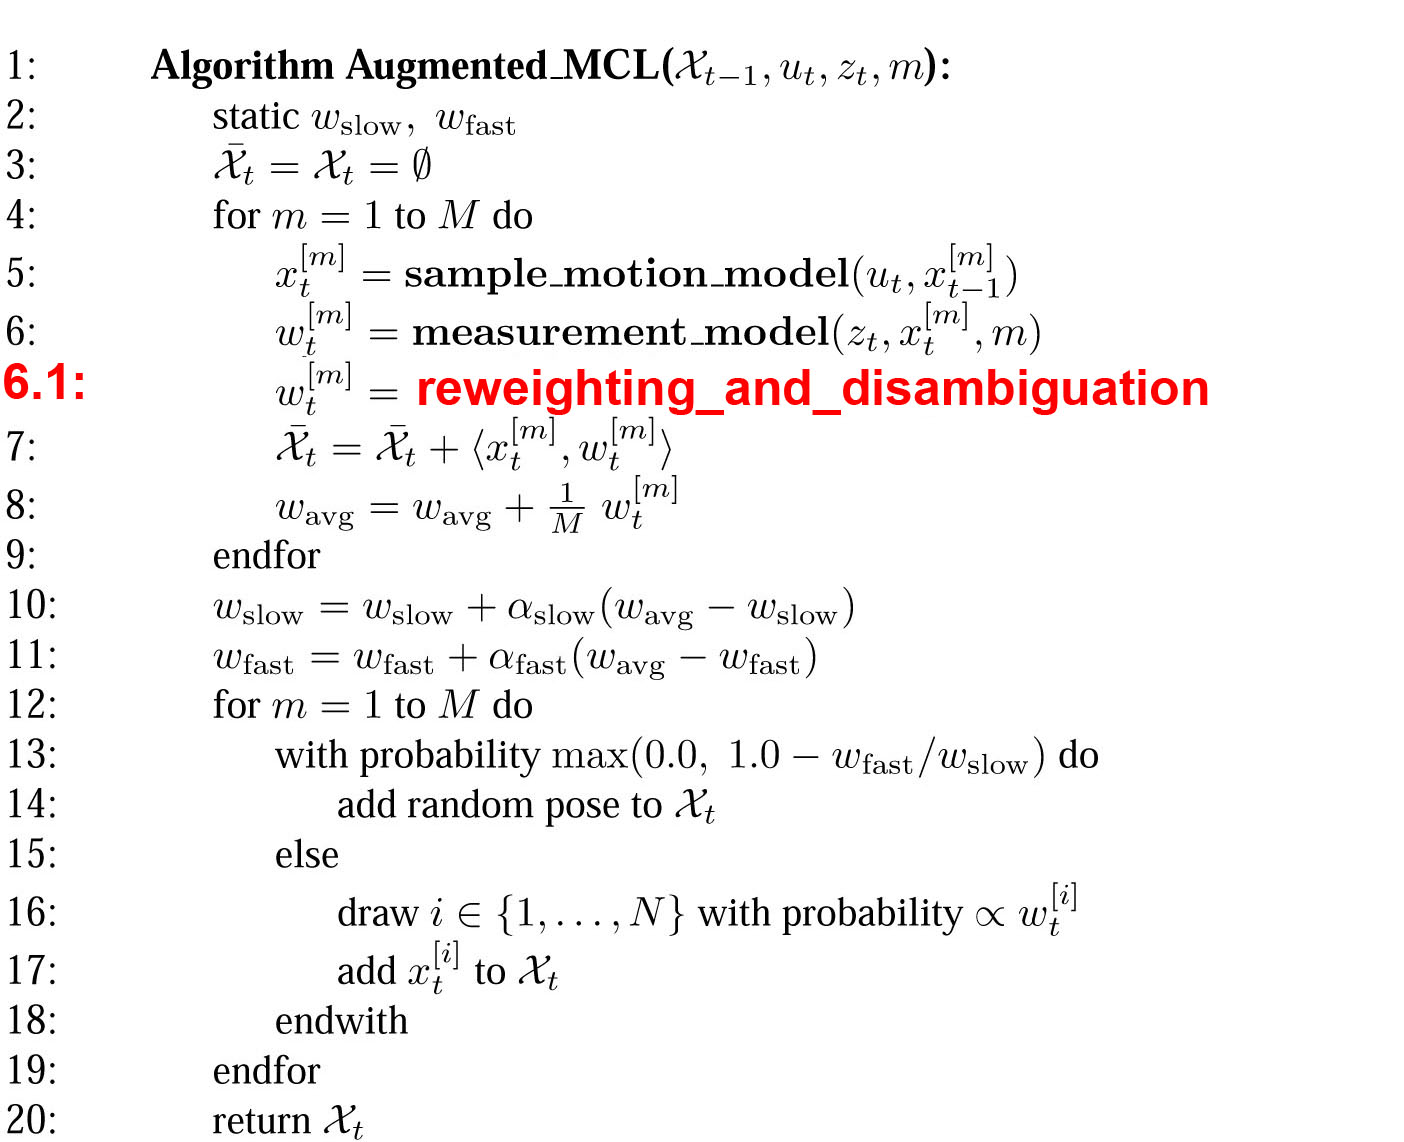
\includegraphics[width=1.2\textwidth]{../Drawings/localisation/MCLAugmented.jpg}
    \caption{The proposed implementation of the method in the Monte Carlo Algorithm \cite{Thrun2002}}
    \label{fig:mclProposed}
\end{minipage}
\end{figure}


\section{Proposed Modification}
\label{sec:modification}
The proposed modification is to add an extra re-weighting routine to the AMCPF algorithm as shown in \figref{fig:mclProposed}. This routine entitled \textit{Reweighting and Disambiguation} will only be called when the robot re-enters the football field after serving a penalty ban. The observations $z_t$ for this routine will be the interest point descriptors computed using the feature extraction algorithm. Once the robot has been able to disambiguate its position, then the AMCPF algorithm will return to its normal operation as shown in \figref{fig:augmented}.\\

\section{Localisation using Natural Visual Landmarks}
\label{sec:localisationNaturalVisualLandmarks}
The localisation algorithm is broken down into a number of sub-routines. These include the initialisation routine, the re-localisation procedure on re-entering the field, the descriptor matching and finally disambiguation.\\

\section{Initialisation Routine}
\label{sec:initialisation}
The first step in localising the robot occurs prior to the start of the game. The robot will initially capture a set of $m$ images of regions behind each of the goal posts. The interest points will be detected using the feature extraction algorithm for each image and descriptors for these interest points will be computed and stored by the robot for the remainder of the game. These descriptors represent the visual landmarks and the set of computed descriptors will be referred to as $d_{initial}^i |i = 1,2...m$ where $i$ represents the image number. It is assumed that these visual landmarks are persistent throughout the game. However, this is the initial proposal and the features can be updated during the course of the game as a future addition.\\

\section{Re-localisation Procedure}
\label{sec:relocalisation}
When a penalty occurs and a robot is removed from the field, it has to relocalise itself on re-entering the field after it has served the penalty ban. As mentioned previously, the robot is placed on the half-way line, the nearest spot from the half-way line or on its respective side of the field facing the opposition once the penalty period has ended. The example figures below portray the scenario that occurs when the robot re-enters the pitch from the half-way line on the left-hand side of the field. This will be the example scenario used to describe the algorithm.\\

\textbf{IMAGE OF POSSIBLE POSITIONS}

The robot knows that it re-enters the field on its side of the pitch. However, ambiguities arise as it does not know which position on its side of the pitch it currently occupies as well as its current orientation. At this point, the robot receives a list of visual landmarks that are present on the football field. These include the goal posts, line segments, line crossings (intersections between line segments) and the center circle \cite{Bhuman}. These are illustrated in \figref{fig:localiseLandmarks}. Using these visual landmarks, the AMCPF algorithm re-weights the particles and the robot knows that it is in one of two locations due to the symmetrical nature of the football field. The possible locations are illustrated in \figref{fig:before} and \figref{fig:beforeSim}. \figref{fig:beforeSim} is a screenshot from the \textit{BHuman SimRobot Simulator} \cite{Bhuman}. As can be seen in the figures, each potential location is represented by a dense cluster of particles. In addition, random particles will also be present due to the particle injection property of the algorithm.\\

\begin{figure}[ht!]
  \centering
    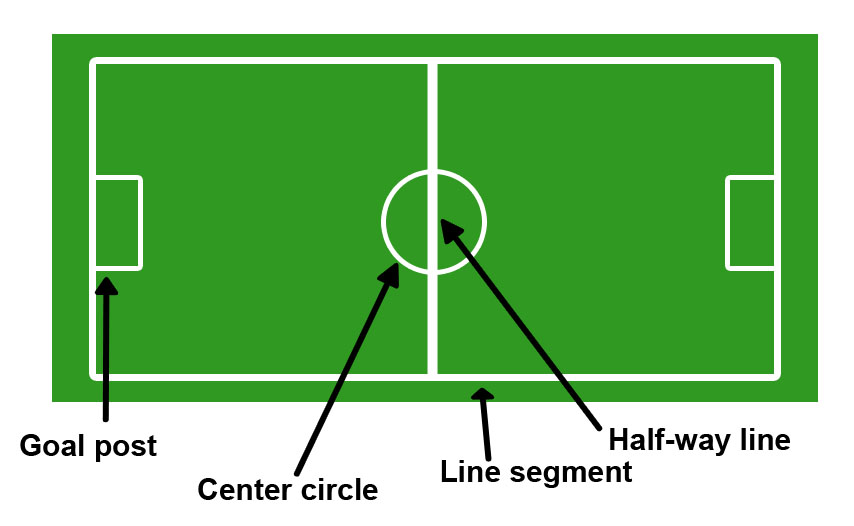
\includegraphics[width=0.4\textwidth]{../Drawings/localisation/goalSetup.jpg}
    \caption{The visual landmarks available on the football field} 
    \label{fig:localiseLandmarks}
\end{figure}

\begin{figure}[ht!]
\begin{minipage}[b]{0.5\linewidth}
  \centering
    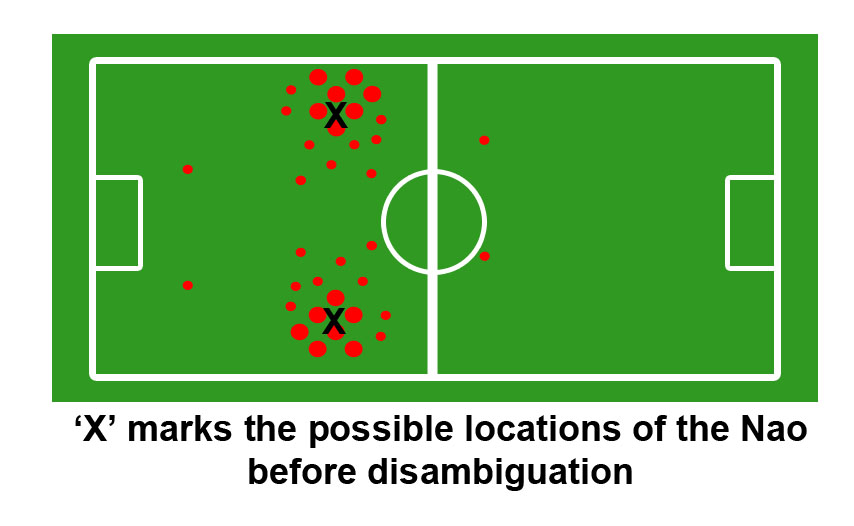
\includegraphics[width=0.6\textwidth]{../Drawings/localisation/beforeDisambiguate.jpg}
    \caption{Two possible positions are surrounded by particles with large weights.} 
    \label{fig:before}
\end{minipage}
\begin{minipage}[b]{0.5\linewidth}
  \centering
    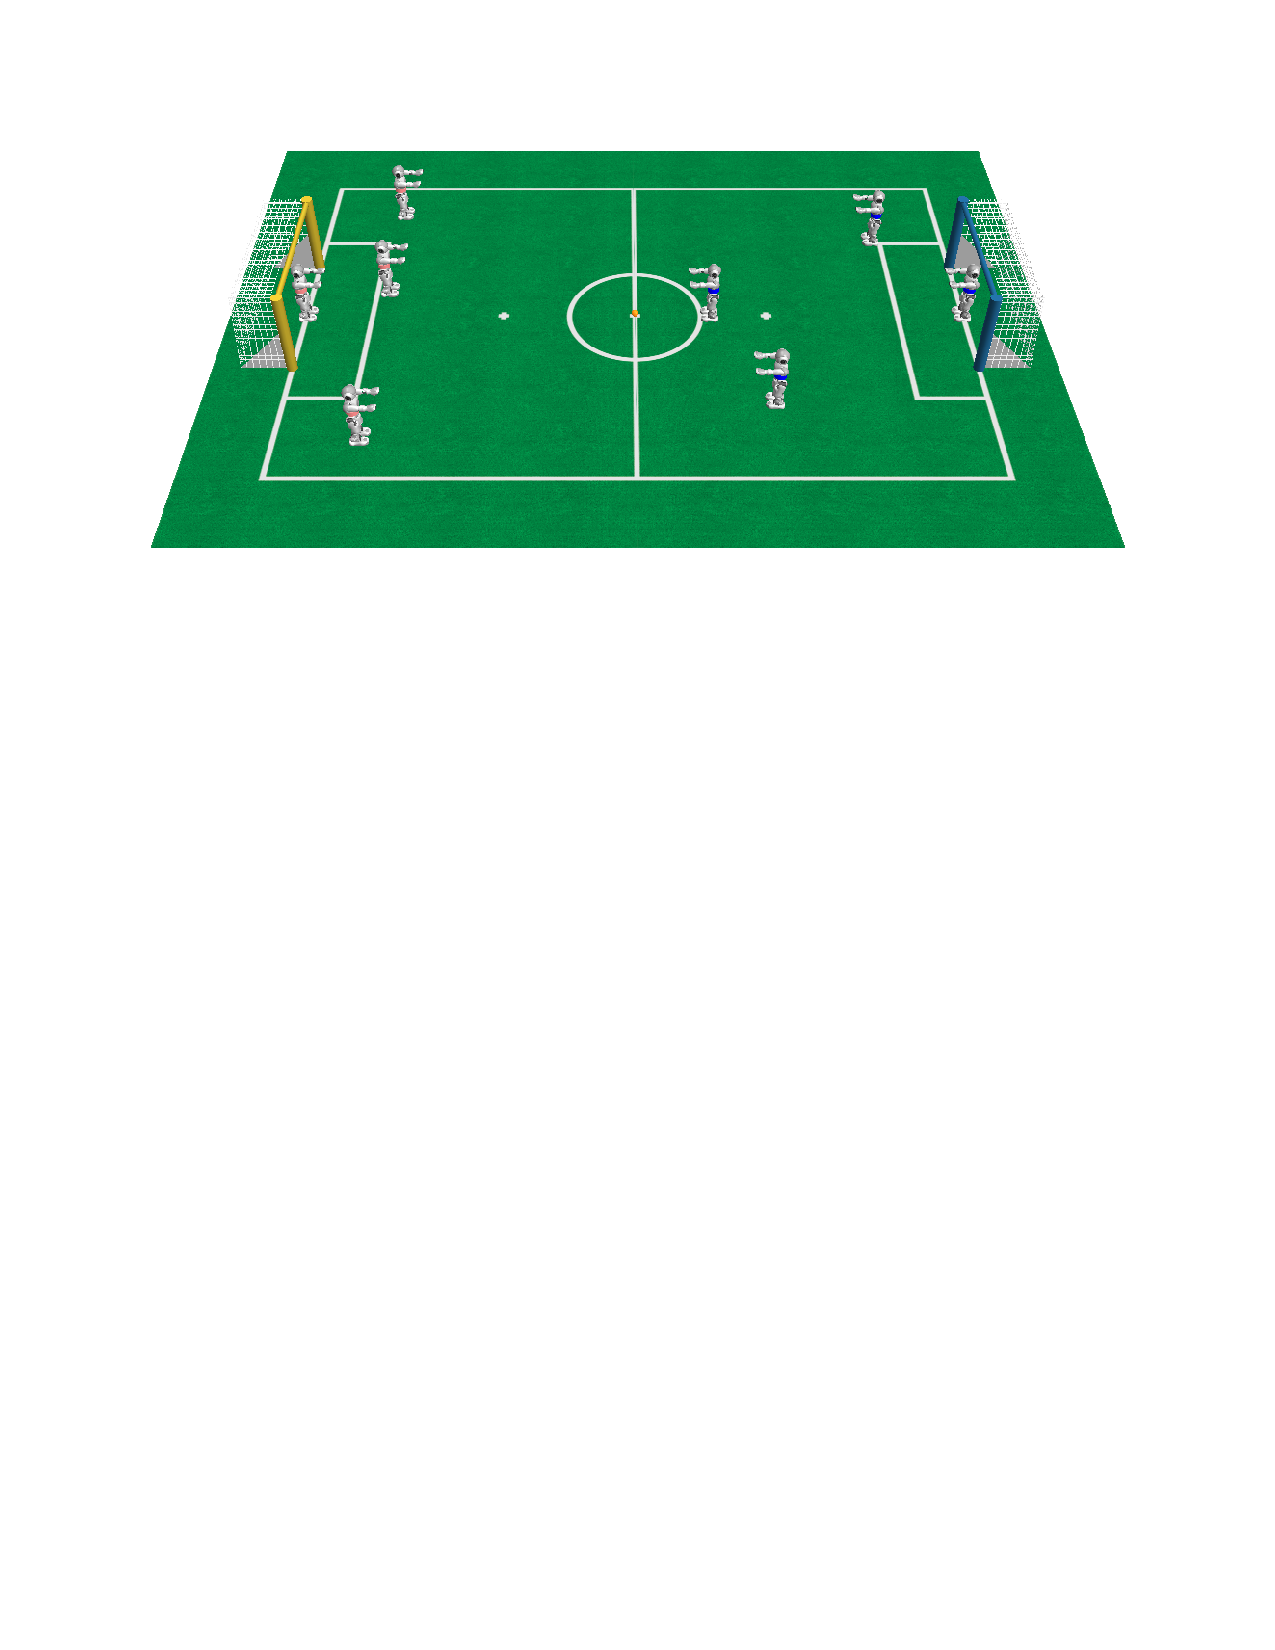
\includegraphics[width=0.5\textwidth]{../Drawings/localisation/NaoField.jpg}
    \caption{The SimRobot simulation of the particles on re-entering the field}
    \label{fig:beforeSim}
\end{minipage}
\end{figure}


%Disambiguation step
%Discuss when it comes onto the field.
\section{Descriptor Matching}
\label{sec:disambiguation}
It is at this point that the proposed modification to the localisation algorithm will be utilised. It should be noted that each particle has an $(x,y)$ position and an orientation $\theta$. It is the particle's orientation $\theta$ that is crucial to this algorithm working effectively. As can be seen in \figref{fig:penaltyOver}, the robot has re-entered the pitch and the particles are given random orientations. The robot will then rotate its head counter-clockwise (arbitrarily chosen) to face the left goal post as shown in \figref{fig:turnedLeft}. Both clusters of particles will rotate counter-clockwise by the same angle. Due to the symmetry of the environment, the correct cluster will rotate in the same direction as the robot's head whereas the incorrect cluster will rotate in the opposite direction.\\

The robot will then utilise its feature extraction algorithm to identify interest points in regions behind the respective goal post that it is facing. This scenario is shown in \figref{fig:featureMatching} where the robot has identified interest points $F1, F2, F3$. Descriptors for these interest points will then be computed and the set of descriptors will be referred to as $d_{current}^c$ where $c$ is the current image.

The algorithm will then match the current descriptors from $d_{current}^c$ with descriptors from $d_{initial}^j|j=1,2...m$. The set of descriptors, $d_{initial}^j$, corresponding to the best match with $d_{current}^c$, will determine the goal post which the robot is currently facing. This can be seen in the figure whereby the robot has matched its current descriptors to the stored descriptors relating to the image of the robot's goal post. In this example, the robot knows from matching the descriptors that it is therefore facing its goalpost.\\
 
\begin{figure}[ht!]
\begin{minipage}[b]{0.5\linewidth}
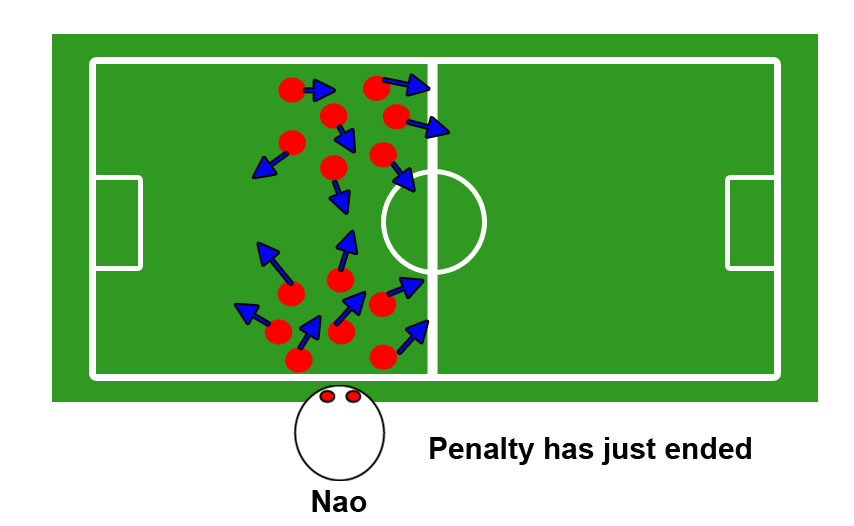
\includegraphics[scale=0.2]{../Drawings/localisation/localisationAlgorithmPenaltyEnded.jpg}
\caption{The particles representing hypotheses of the possible robot position after the robot has served its penalty time.}
\label{fig:penaltyOver}
\end{minipage}
\hspace{0.5cm}
\begin{minipage}[b]{0.5\linewidth}
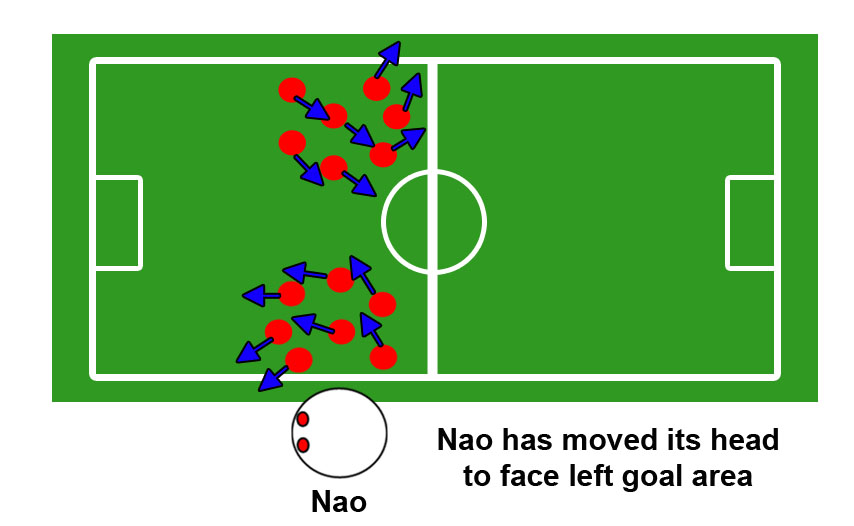
\includegraphics[scale=0.2]{../Drawings/localisation/localisationAlgorithmTurnedLeft.jpg}
\caption{The robot turns its head to the left and the orientations of the particles change accordingly.}
\label{fig:turnedLeft}
\end{minipage}
\end{figure}

%Matching interest point descriptors
\begin{figure}[h!] 
  \centering
    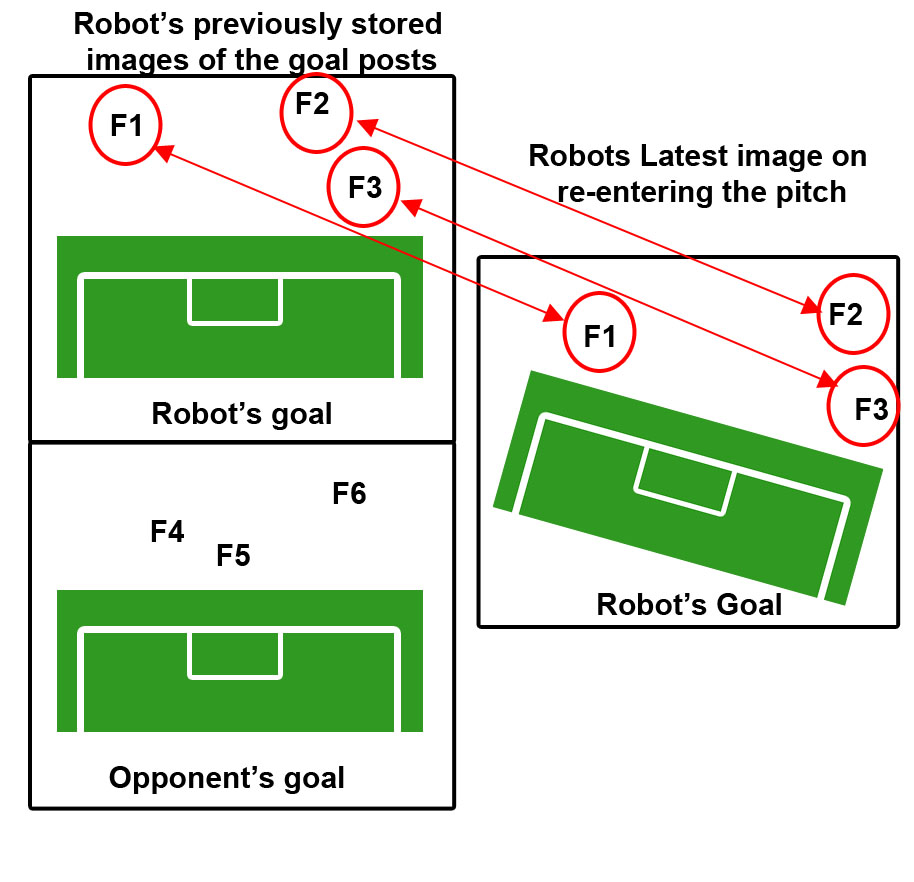
\includegraphics[width=0.5\textwidth]{../Drawings/localisation/featureMatching.jpg}
    \caption{Matching interest point descriptors to disambiguate the robot's position}
    \label{fig:featureMatching}
\end{figure}



\section{Re-weighting Procedure}
\label{sec:reweighting}
The algorithm will be able to disambiguate the robots position on the field by re-weighting the particles in the AMCPF algorithm. The re-weighting procedure is performed as follows. The algorithm knows the robots current head orientation $\beta$. All particles whose current orientation is $\beta -\frac{\pi}{2} \leq \theta \leq \beta + \frac{\pi}{2}$ will be assigned a large weight as these particles are most likely clustered around the robot's true position. All other particles will be assigned a low weight. This should result in the robot being able to disambiguate its position as seen in \figref{fig:reweight}. Once this has been achieved, the AMCPF algorithm returns to its normal operation which only re-weights particle using visual landmarks shown in \figref{fig:localiseLandmarks}. If some incorrect particles are assigned large weights, then they will quickly disappear in subsequent re-weighting procedures since the particle's position and orientation hypothesis will not coincide with the observations that the robot receives from the field.\\


%Leading up to the final state
\begin{figure}[h!] 
\centering
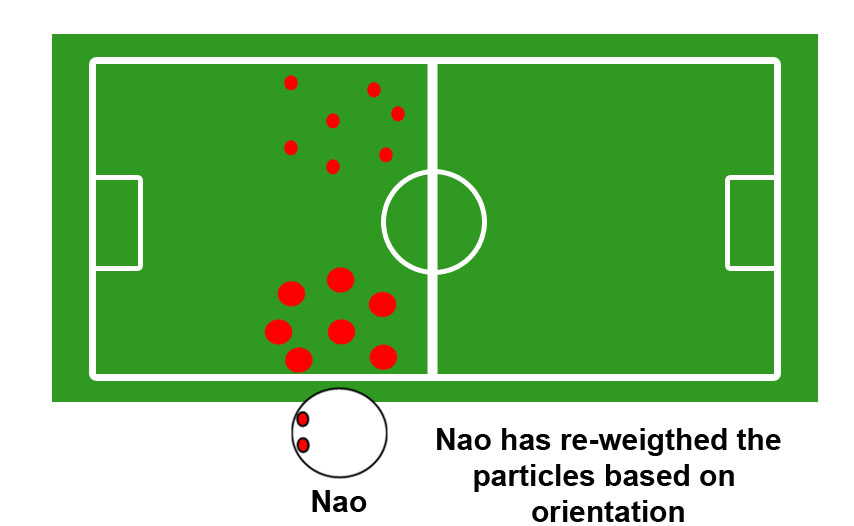
\includegraphics[scale=0.2]{../Drawings/localisation/localisationAlgorithmReweight.jpg}
\caption{The robot then re-weights the particles that have approximately the same orientation as the robot.}
\label{fig:reweight}
\end{figure}

%The final state
%\begin{figure}[h!] 
%  \centering
%    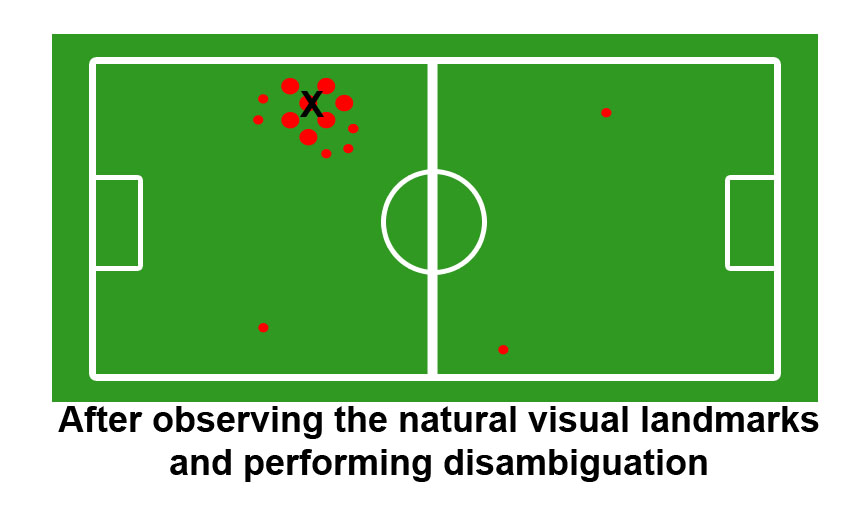
\includegraphics[width=0.5\textwidth]{../Drawings/localisation/afterDisambiguate.jpg}
%    \caption{The robot's estimated position after disambiguation}
%    \label{fig:after}
%\end{figure}




%Discuss how the robot performs the localisation procedure.
%Briefly mention the fact that the robot relocalises itself using a re-weighting routine
%
%\section{Re-weighting Particles and Importance Sampling}
%\label{sec:reweighting}
%This is where the orientation algorithm is placed



%\section{Bhuman Code Structure}
%\label{sec:codeStructure}
%Discuss the basics of the bhuman code structure
%Include a basic diagram of modules, representations etc

%\section{Natural Landmark Code Structure}
%\label{sec:naturalLandmarkCode}
%Discuss how the Natural landmark detection has been placed into the bhuman code structure
%include a diagram from the simRobot interface

\section{Summary}
\label{sec:summary4}